\documentclass[runningheads]{llncs}

\usepackage{amssymb,amsmath,mathtools,empheq,fancybox}

\usepackage{paralist}
\usepackage{url}
\usepackage{color}

\usepackage{textcomp,listings}
\usepackage{biblatex}
\usepackage{mymacros}
\usepackage{mathpartir}
\addbibresource{../bibliography.bib}



\newif\ifcomments
\commentstrue

\newcommand{\pr}[1]{{\color{red}``PR: #1''}}
\newcommand{\as}[1]{{\color{blue}``AS: #1''}}

\newif\ifoutline
\outlinetrue

\newcommand{\contents}[1]{\ifoutline{\color{blue}
    \begin{itemize}
    #1
    \end{itemize}
  }\fi}

\allowdisplaybreaks[1]

\title{A Solver for Generalised Parikh Images of Conjunctions of Regular Languages}
\author{some cool authors}
\institute{Uppsala University, Sweden}

\begin{document}
\maketitle

\section{Introduction}

Parikh maps and their image appears naturally as part of many operations in
model checking and the solving of string constraints in automata-based string
solvers such as \Ostrich{} \cite{ostrich}. While it is possible to compute the Parikh image of
an automaton using the method described in \cite{generate-parikh-image}, this
method produces large existentially quantified clauses which are costly to
eliminate and in practice make many real-world problems intractable.
Furthermore, many modern applications require automata with symbolic labels to
handle large alphabets, which has no immediate correspondence in the methods described. Automata-based string solvers like \Ostrich{} also compute
Parikh images on products of automata, derived from conjunctions of string
constraints. Under previous methods this would require the computation of the
product before the Parikh image can be computed, running the risk of an
exponential blow-up.

Addressing these concerns, our approach allows us to extend the computation of
Parikh images to handle symbolic transition labels naturally, while also
allowing us to interleave the computation of arbitrarily deep products of
automata with the Parikh image of their product. This allows us to let both
calculations inform each other, allowing the computation of partial products to
inform the computation of the product and vice versa. Moreover, the scheme
allows us to learn interesting facts (implied clauses) about the problem.

Based on these insights, we present a tool to solve linear constraints on
symbolic automata with counters, amounting to constraints on the Parikh image of
their product. We are able to generate symbolic as well as concrete Parikh images.

\section{Background}

Formally, the \textit{Parikh map} over a context-free language $\Sigma = \left\{a_1, \ldots, a_k \right\}$ is defined as in \cite{kozen}:

$$
\begin{aligned}
& \psi: \Sigma^* \rightarrow \mathbb{N}^k \\
& \psi(s) = \left[\#a_1(s), \#a_2(s), \ldots, \#a_k(s)\right]
\end{aligned}
$$

That is, $\psi(s)$ is a vector of the number of occurrences of each character in the language for a given string $s$. For example, for  $\Sigma = \left \{ a, b\right\}$, we would have $\psi(abb) = \left[1, 2\right]$.

We define the image of this map, the \textit{Parikh image}, of some subset of the language $A \subseteq \Sigma^*$ as:

$$
\psi(A) = \left\{ \psi(x) | x \in A \right\}
$$

Thus we would have $\psi(\left\{ab, abb\right\}) = \left\{\left[1, 1\right], \left[1, 2\right]\right\}$.

\subsection{Generalised Parikh Images}\label{sec:generalised}

Another way of viewing the Parikh map is as a monoid homomorphism $p:\: \left(\Sigma^*, \cdot, \epsilon \right) \to (\mathbb{Z}^\Sigma, +, \vec{0})$, where $\cdot$ is the string concatenation operation, the objects of the right-hand-side monoid are character counts, and $+$ is standard vector addition. Note that while the left monoid does not commute, the right one does.

This viewpoint enables us to generalise the Parikh map and its image further to arbitrary monoid morphisms $h:\: \Sigma^* \to M$ where $M$ is a commutative monoid. It then follows from the universal mapping property that any such morphism $h$ can also be expressed in terms of the Parikh map, as $h' \circ p$.

A useful example of such a morphism might be computing the length of a string,
which could be recast in terms of the Parikh map by summing the individual
character counts of the vector: $h':\: (\mathbb{Z}^\Sigma, +, \vec{0}) \to
(\mathbb{Z}, +, 0) = \vec{x} \to \sum_{i \in \Sigma} x_i$, where the respective
operators $+$ is element-wise vector addition and integer addition respectively.
This allows us to apply selective logics, symbolic logics, and arithmetic on
counter variables to the Parikh image calculus.

\section{Lazy Computation of Parikh Images for Regular Languages}

Starting with the automaton in~\ref{fig:start}, we seek any value in its Parikh image, i.e. a character count.

\begin{figure}[h]
  \centering
  \label{fig:start}
  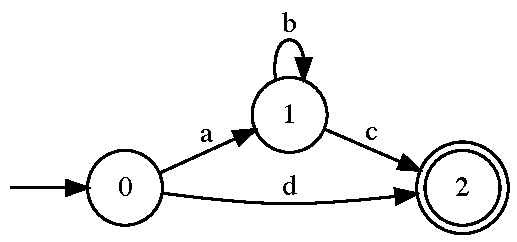
\includegraphics[width=0.5\textwidth]{trace-0}
  \end{figure}

  In this case, our calculation will introduce a free (and fresh) integer constant per character ($a$, $b$, $c$, and $d$). It will then start by introducing equations preserving flow through the automaton corresponding to how many times that transition is used in a path from the initial state to an accepting state. Each transition will be given an existentially quantified variable in these equations, and each of our target variables set equal to the sum of their corresponding transitions. This corresponds to the first portion of the formula described in~\cite{generate-parikh-image}, but crucially misses the constraints to ensure connectivity of a path in the presence of cycles. Instead, we enforce these constraints lazily using our own calculus rules to.
  
  Note that this formulation allows us to propagate information between the terms of the product without (and before) computing the full product. For many unsatisfiable instances, this corresponds to the method recently introduced in~\cite{approximate-parikh}, where the Parikh-image of a product of automata is over-approximated to the conjunction of their Parikh images.
  
Before computation using our rules begin, our automated theorem prover performs reasoning on the linear flow equations to simplify them into:
$$
\exists_{x_{0}} : d + a = 1 \land
c = a
$$

Note the disappearance of all but one of the transition variables and their replacement with the corresponding linear equations:

\begin{figure}[h]
  \centering
  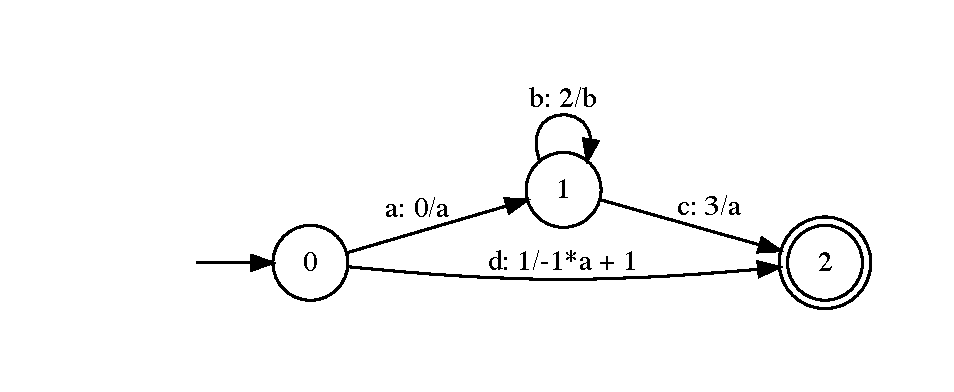
\includegraphics[width=\textwidth]{trace-0-aut-0}
\end{figure}
  
We now have a choice of two paths through the automaton and execute a case split: \textsc{Split}: $a \leq 0$ $\mid$ $a > 0$. The split is performed as close to the initial state as possible and favours deselecting an edge by constraining its corresponding term to be 0.

Since this decision disconnects a loop, the $b$~transition, from the initial state, we evaluate the rule \textsc{Propagate-Connected} and add the constraint $b = 0$. Following this, we can also subsume the propagating machinery for the connectedness constraint, as there are no nonzero loop transitions left. This leaves us with an automaton with just one nonzero transition, as in figure~\ref{fig:final}.

\begin{figure}[h]
  \centering
  \label{fig:final}
  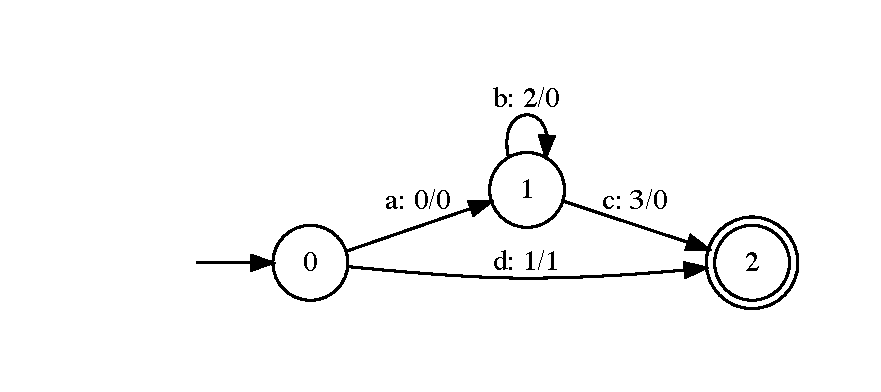
\includegraphics[width=\textwidth]{trace-3-aut-0}
  \end{figure}
  

Since this automaton is trivially connected and allows for only one solution, we
present the solution $a = b = c = 0, d=1$.

\section{Possible Applications}
Bring your own!


%\bibliographystyle{splncs03}
\printbibliography

\end{document}
